% Drawing 148/02-1 -- folder 148, batch 02, archive page 22 (PDF page 23).
% Transcription: sous ces mots, un croquis d'un prisme ou d'une pyramide carrée, au crayon et à l'encre ; puis un petit parallélogramme dont un sommet est marqué, et, à côté :
% Kind: sketch of a prism or square pyramid; parallelogram with marked vertex. Method 2 (schematic redraw from the facsimile). Status: partial.
% Notes: Re-read on a colour crop of p. 22. Under "Carre oriente": a sketch of a solid with an apex joined to three points and a lower vertex, ink strokes (some doubled) and pencil strokes; one edge (left vertex to the middle right vertex) is red-brown, and a red-brown arc runs down the right of the sketch. Below, a parallelogram whose upper left vertex is a heavy point and lower right vertex an open point, with a curved rotation arrow over the marked vertex. Which solid is meant (prism or square pyramid) is not decided by the drawing, and the pencil strokes are approximate.
% Coordinates: 1 unit = 1 mm = 1/100 of the crop width (bbox in page fractions: [0.15, 0.59, 0.46, 0.77]).
% Redrawn by Claude (claude-opus-5-5), issue #73, 2026-11-07; not checked by a human; not compiled (no TeX in the session).
% Rights: reproduces part of the work -- behind RENDER_TRANSCRIPTS, never published by itself.
\documentclass[tikz,border=3pt]{standalone}
\usepackage{amsmath,amssymb}
\usetikzlibrary{patterns,arrows.meta}
\tikzset{Rd/.style={red!85!black}, pencil/.style={black!45}, struck/.style={black!35}, mark/.style={circle,draw,inner sep=1.3pt}, pt/.style={circle,fill,inner sep=0.9pt}, opt/.style={circle,draw,fill=white,inner sep=1.1pt}}
\begin{document}
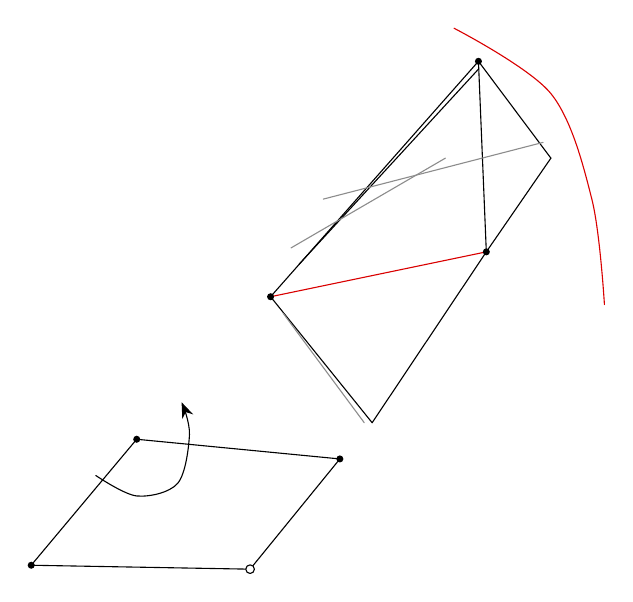
\begin{tikzpicture}[x=1mm,y=1mm,line cap=round,line join=round,font=\scriptsize]
\draw (82.5,-8.9) -- (56.1,-38.8);
\draw (82.5,-9.9) -- (59.7,-34.7);
\draw (82.5,-8.9) -- (83.5,-33.1);
\draw (82.5,-8.9) -- (91.7,-21.2);
\draw (91.7,-21.2) -- (83.5,-33.1) -- (69,-54.8);
\draw (56.1,-38.8) -- (69,-54.8);
\draw[pencil] (57.7,-40.9) -- (68,-54.8);
\draw[Rd] (56.1,-38.8) -- (83.5,-33.1);
\draw[pencil] (58.7,-32.6) -- (78.3,-21.2);
\draw[pencil] (62.8,-26.4) -- (90.7,-19.2);
\draw[Rd] plot[smooth, tension=0.55] coordinates {(79.4,-4.7) (91.7,-13) (96.9,-26.4) (98.5,-39.8)};
\node[pt] at (82.5,-8.9) {};
\node[pt] at (56.1,-38.8) {};
\node[pt] at (83.5,-33.1) {};
\draw (39.1,-56.9) -- (64.9,-59.4) -- (53.5,-73.4) -- (25.7,-72.9) -- cycle;
\node[pt] at (39.1,-56.9) {};
\node[pt] at (64.9,-59.4) {};
\node[pt] at (25.7,-72.9) {};
\node[opt] at (53.5,-73.4) {};
\draw[-{Stealth[length=2mm]}] plot[smooth, tension=0.55] coordinates {(33.9,-61.5) (39.1,-64.1) (44.3,-62.5) (45.8,-56.3) (44.8,-52.2)};
\end{tikzpicture}
\end{document}
